\documentclass[
	9pt, % Set the default font size, options include: 8pt, 9pt, 10pt, 11pt, 12pt, 14pt, 17pt, 20pt
	t, % Uncomment to vertically align all slide content to the top of the slide, rather than the default centered
	%aspectratio=169, % Uncomment to set the aspect ratio to a 16:9 ratio which matches the aspect ratio of 1080p and 4K screens and projectors
]{beamer}

\graphicspath{{Images/}{./}} % Specifies where to look for included images (trailing slash required)

\usepackage{booktabs} % Allows the use of \toprule, \midrule and \bottomrule for better rules in tables
\usepackage{graphicx}
\usepackage{caption}
\usepackage{subcaption}
\usepackage{hyperref}
\usepackage[english,brazil]{babel}
\usepackage{fontawesome5}
\usepackage{listings}
\usepackage{minted}
\usepackage{xcolor}
% \usepackage{graphicx}
% \usepackage{animate}
\RequirePackage[backend=biber,
	style=ieee,
	citestyle=authoryear,
]{biblatex}

% Define a custom command for an icon link
\newcommand{\iconLink}[2]{\href{#1}{\faLink \hspace{0.2em} {#2}}}
\newcommand{\yellowbox}[1]{\colorbox{yellow!75}{#1}}

% Definindo um estilo para o destaque
%----------------------------------------------------------------------------------------
%	SELECT LAYOUT THEME
%----------------------------------------------------------------------------------------
\usetheme{Madrid}

%----------------------------------------------------------------------------------------
%	SELECT COLOR THEME
%----------------------------------------------------------------------------------------

% Beamer comes with a number of color themes that can be applied to any layout theme to change its colors. Uncomment each of these in turn to see how they change the colors of your selected layout theme.

%\usecolortheme{albatross}
%\usecolortheme{beaver}
%\usecolortheme{beetle}
% \usecolortheme{crane}
%\usecolortheme{dolphin}
%\usecolortheme{dove}
%\usecolortheme{fly}
%\usecolortheme{lily}
%\usecolortheme{monarca}
%\usecolortheme{seagull}
%\usecolortheme{seahorse}
%\usecolortheme{spruce}
%\usecolortheme{whale}
%\usecolortheme{wolverine}

%----------------------------------------------------------------------------------------
%	SELECT FONT THEME & FONTS
%----------------------------------------------------------------------------------------
\usefonttheme{default} % Typeset using the default sans serif font

%------------------------------------------------

\usepackage{palatino} % Use the Palatino font for serif text
\usepackage[default]{lato} % Use the Lato font for sans serif text

%----------------------------------------------------------------------------------------
%	SELECT INNER THEME
%----------------------------------------------------------------------------------------
\useinnertheme{rectangles}

%----------------------------------------------------------------------------------------
%	SELECT OUTER THEME
%----------------------------------------------------------------------------------------

% Outer themes change the overall layout of slides, such as: header and footer lines, sidebars and slide titles. Uncomment each theme in turn to see what changes it makes to your presentation.

%\useoutertheme{default}
%\useoutertheme{infolines}
%\useoutertheme{miniframes}
%\useoutertheme{smoothbars}
%\useoutertheme{sidebar}
%\useoutertheme{split}
%\useoutertheme{shadow}
%\useoutertheme{tree}
%\useoutertheme{smoothtree}

%\setbeamertemplate{footline} % Uncomment this line to remove the footer line in all slides
%\setbeamertemplate{footline}[page number] % Uncomment this line to replace the footer line in all slides with a simple slide count

%\setbeamertemplate{navigation symbols}{} % Uncomment this line to remove the navigation symbols from the bottom of all slides

% \bibliography{references} % Specifies the bibliography file to include publications
% \bibliographystyle{apalike} % Specifies the bibliography style
\addbibresource{references.bib}

%----------------------------------------------------------------------------------------
%	PRESENTATION INFORMATION
%----------------------------------------------------------------------------------------

\title[DesWebII]{Desenvolvimento Web II} % The short title in the optional parameter appears at the bottom of every slide, the full title in the main parameter is only on the title page
\subtitle{Aula 04 - Web Service e API} % Presentation subtitle, remove this command if a subtitle isn't required
\author[Fabricio Bizotto]{Prof. Fabricio Bizotto} % Presenter name(s), the optional parameter can contain a shortened version to appear on the bottom of every slide, while the main parameter will appear on the title slide
\institute[IFC]{Instituto Federal Catarinense \\ \smallskip \textit{fabricio.bizotto@ifc.edu.br}} % Your institution, the optional parameter can be used for the institution shorthand and will appear on the bottom of every slide after author names, while the required parameter is used on the title slide and can include your email address or additional information on separate lines
\date[\today]{Ciência da Computação \\ \today} % Presentation date or conference/meeting name, the optional parameter can contain a shortened version to appear on the bottom of every slide, while the required parameter value is output to the title slide

%----------------------------------------------------------------------------------------
\begin{document}

%----------------------------------------------------------------------------------------
%	TITLE SLIDE
%----------------------------------------------------------------------------------------

\begin{frame}
	\titlepage % Output the title slide, automatically created using the text entered in the PRESENTATION INFORMATION block above
\end{frame}

%----------------------------------------------------------------------------------------
%	TABLE OF CONTENTS SLIDE
%----------------------------------------------------------------------------------------

\begin{frame}
	\frametitle{Roteiro} % Slide title, remove this command for no title

	\tableofcontents % Output the table of contents (all sections on one slide)
	%\tableofcontents[pausesections] % Output the table of contents (break sections up across separate slides)
\end{frame}

%----------------------------------------------------------------------------------------
%	PRESENTATION BODY SLIDES
%----------------------------------------------------------------------------------------

\section{Web Service} % Sections are added in order to organize your presentation into discrete blocks, all sections and subsections are automatically output to the table of contents as an overview of the talk but NOT output in the presentation as separate slides

%------------------------------------------------

\begin{frame}
	\frametitle{Web Service}

	\begin{block}{Definição}
		\begin{itemize}
			\item É uma solução utilizada na integração de sistemas e na comunicação entre aplicações diferentes.
			\item Permite que aplicações se comuniquem independentemente de linguagem, software e
			      hardware utilizados.
			\item É uma tecnologia utilizada para \alert{padronizar} e \alert{organizar} a comunicação entre aplicações.
		\end{itemize}
	\end{block}

	\begin{block}{Características}
		\begin{itemize}
			\item \textbf{Interoperabilidade} - Comunicação entre diferentes plataformas.
			\item \textbf{Independência de Linguagem} - Permite a comunicação entre diferentes linguagens de programação.
			\item \textbf{Formato de Mensagem} - Utiliza XML ou JSON.
			\item \textbf{Padrões Abertos} - Utiliza padrões abertos como SOAP e REST.
		\end{itemize}
	\end{block}

\end{frame}

\begin{frame}[plain, c]
	\centering
	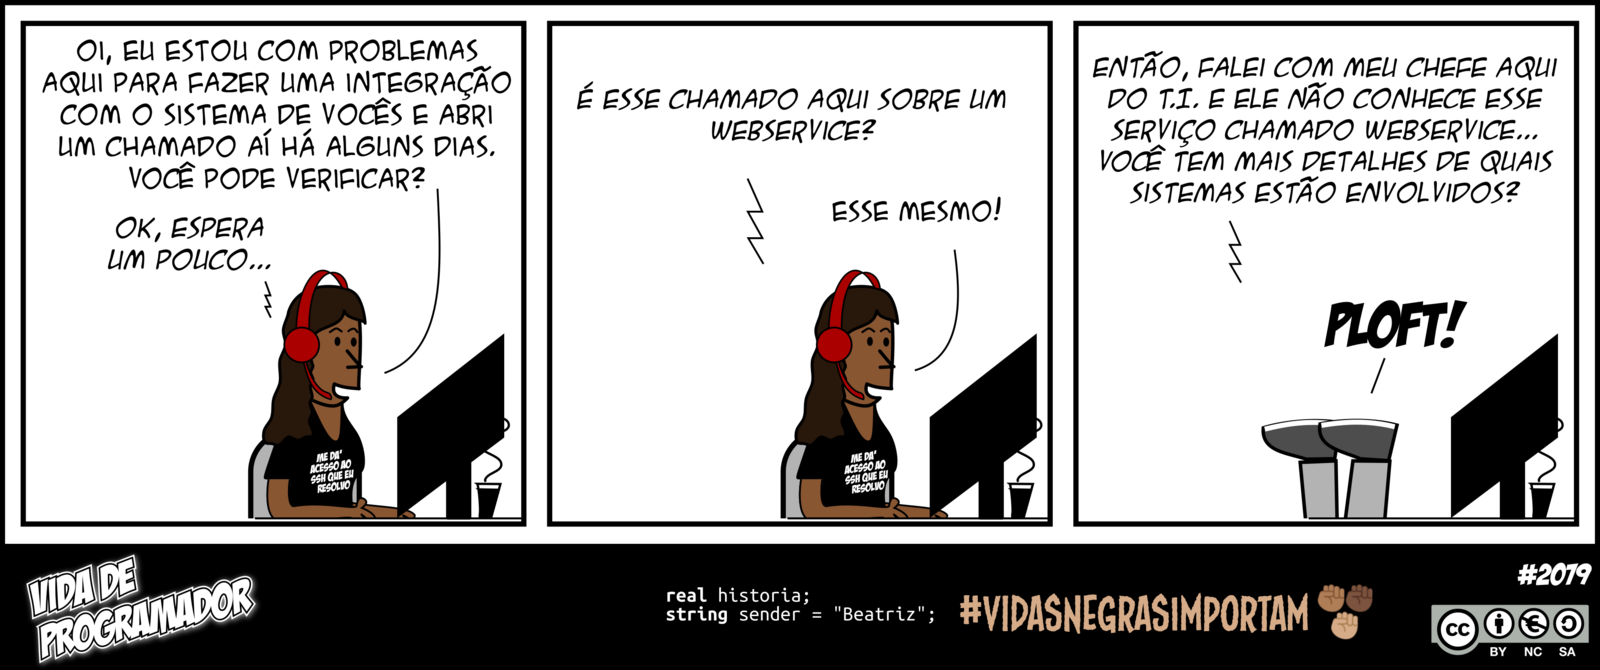
\includegraphics[width=0.9\linewidth]{vdp_ws.png}
\end{frame}

\begin{frame}[plain, c]
	\centering
	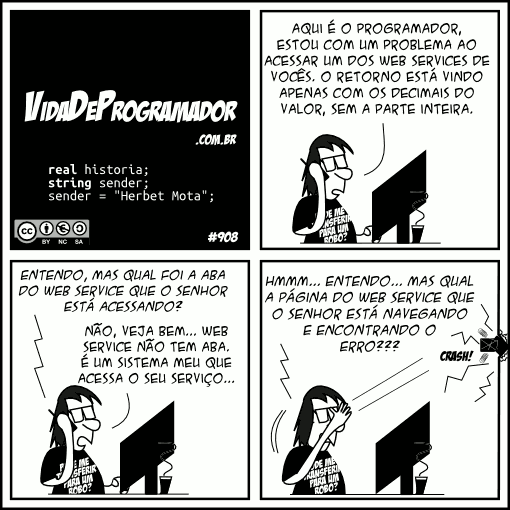
\includegraphics[width=0.7\linewidth]{vdp_ws2.png}
\end{frame}

\begin{frame}
	\frametitle{Web Service}
	\framesubtitle{Web Service vs API}

	\begin{block}{API - \textit{Application Programming Interface}}
		API é um termo bastante amplo, que não necessariamente descreve um web service.
		API é uma interface que permite a comunicação entre dois componentes de software.
		Por meio de uma API, um software cliente é capaz de consumir serviços disponibilizados por um software servidor.
	\end{block}

	\begin{block}{Web Service}
		Um web service, por sua vez, é um tipo de API que fornece a sua interface de comunicação \yellowbox{via internet}.
	\end{block}

	\bigskip

	\begin{center}
		\yellowbox{Nem toda API é um web service, mas todos os web services são APIs.}
	\end{center}

\end{frame}

%------------------------------------------------

\section{SOAP}

\begin{frame}
	\begin{center}

		\bigskip\bigskip\bigskip\bigskip % Vertical whitespace
		{\Large Web Service}

		\bigskip\bigskip % Vertical whitespace
		{\Huge SOAP}

		\smallskip
		{\small \textit{Simple Object Access Protocol}}
	\end{center}

\end{frame}

\begin{frame}
	\frametitle{SOAP}
	\framesubtitle{Definição}

	\begin{block}{Definição}
		\begin{itemize}
			\item Protocolo de comunicação usado para troca de mensagens entre aplicações.
			\item As mensagens SOAP basicamente são \alert{documentos XML} serializados seguindo
			      o padrão W3C enviados em cima de um protocolo de rede como HTTP.
			\item Para descrever os serviços SOAP, é comum utilizar o WSDL (\textit{Web Services
				      Description Language}), um documento XML que define a interface, operações, e
			      protocolos de comunicação.
		\end{itemize}
	\end{block}

	\begin{exampleblock}{Estrutura}
		\begin{itemize}
			\item \textit{Envelope} - Define o início e o fim da mensagem. É o elemento raiz.
			\item \textit{Header} - Define informações adicionais sobre a mensagem. Opcional
			\item \textit{Body} - Define o conteúdo da mensagem. Obrigatório.
			\item \textit{Fault} - Define informações sobre erros. Opcional
		\end{itemize}
	\end{exampleblock}

\end{frame}

\begin{frame}
	\frametitle{SOAP}
	\framesubtitle{Estrutura}

	\begin{figure}
		\centering
		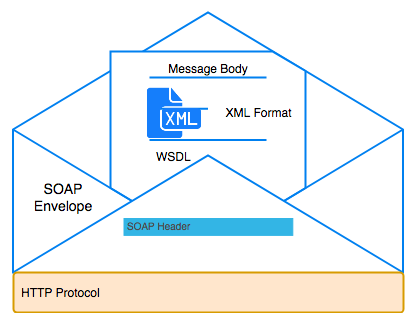
\includegraphics[width=0.7\linewidth]{soap_structure.png}
		\caption{Estrutura SOAP}
		\label{fig:soap}
	\end{figure}

\end{frame}

\begin{frame}
	\begin{center}

		\bigskip\bigskip\bigskip\bigskip % Vertical whitespace
		{\Large Web Service}

		\bigskip\bigskip % Vertical whitespace
		{\Huge SOAP - Exemplo}

		\smallskip
		{\small Requisição e Resposta}
	\end{center}

\end{frame}

\begin{frame}
	\frametitle{SOAP}
	\framesubtitle{Exemplo}

	\begin{figure}
		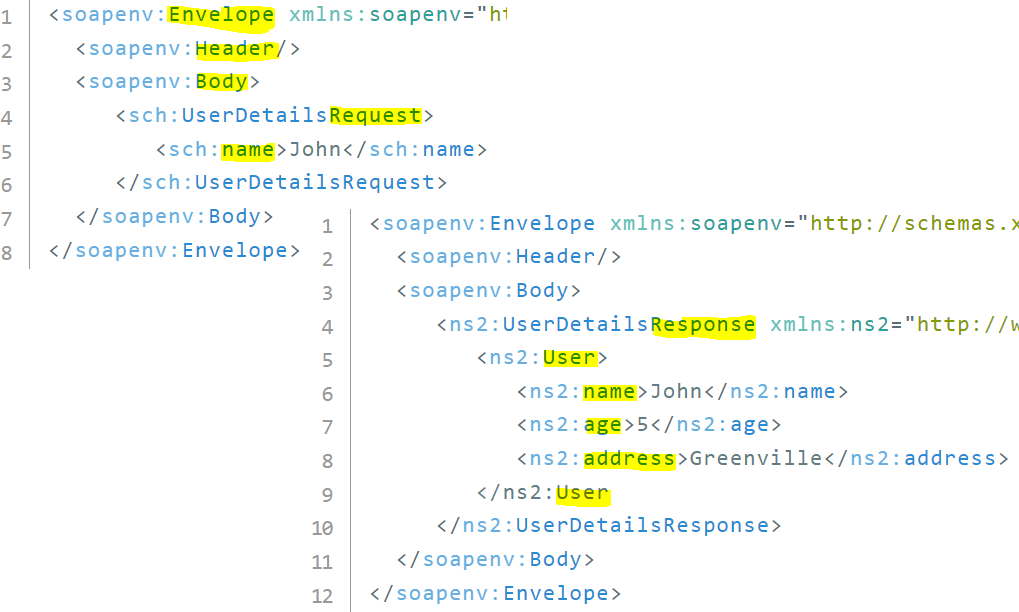
\includegraphics[width=0.8\linewidth]{soap_example_user.png}
		\caption{SOAP - Exemplo - Requisição e Resposta}
		\label{fig:soap_example_user}
	\end{figure}

\end{frame}

\begin{frame}
	\begin{center}

		\bigskip\bigskip\bigskip\bigskip % Vertical whitespace
		{\Large Web Service}

		\bigskip\bigskip % Vertical whitespace
		{\Huge SOAP - Exemplo}

		\smallskip
		{\small Olá Mundo usando protocolo SOAP e Python}
	\end{center}

\end{frame}

\begin{frame}[fragile]
	\frametitle{SOAP}
	\framesubtitle{Servidor}

	\begin{figure}
		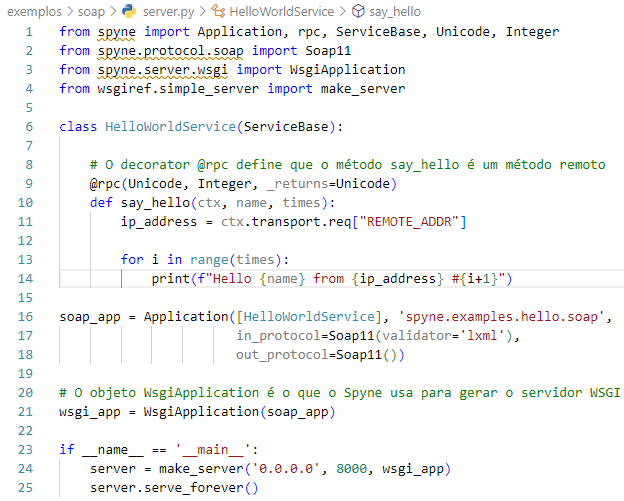
\includegraphics[width=0.7\linewidth]{server_soap.PNG}
		\caption{SOAP - Servidor}
		\label{fig:soap_server}
	\end{figure}

\end{frame}

\begin{frame}[fragile]
	\frametitle{SOAP}
	\framesubtitle{Cliente}

	\begin{figure}
		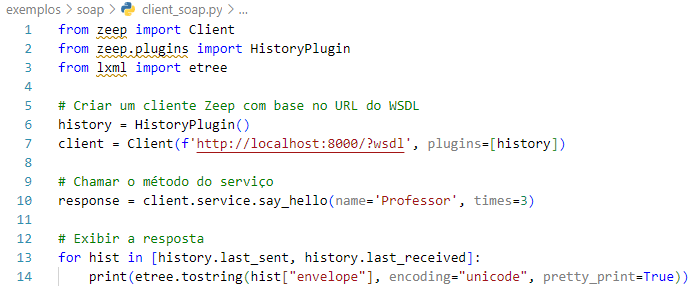
\includegraphics[width=0.9\linewidth]{client_soap.PNG}
		\caption{SOAP - Cliente}
		\label{fig:soap_client}
	\end{figure}

\end{frame}

\begin{frame}[plain, c]
	% \frametitle{SOAP}
	% \framesubtitle{WSDL - \textit{Web Services Description Language}}

	\begin{figure}
		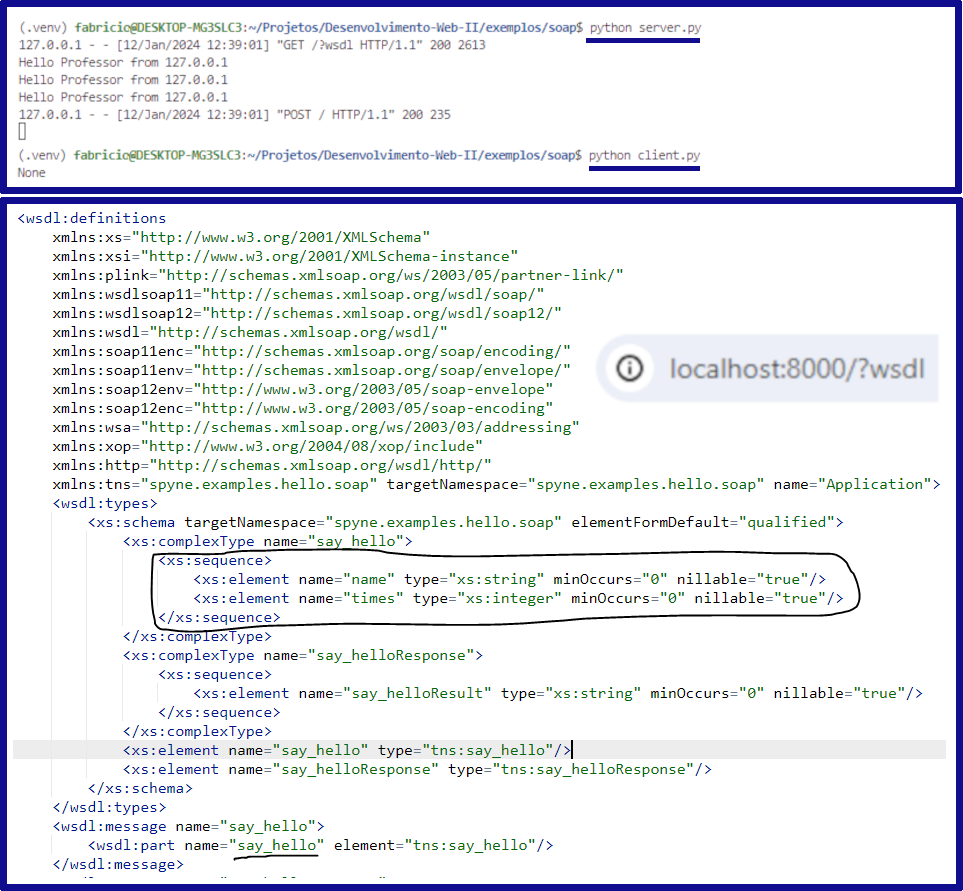
\includegraphics[width=0.75\linewidth]{soap_example.png}
		\caption{SOAP - Chamada e WSDL}
		\label{fig:soap_example}
	\end{figure}

\end{frame}

\begin{frame}
	\begin{center}

		\bigskip\bigskip\bigskip\bigskip % Vertical whitespace
		{\Large Web Service}

		\bigskip\bigskip % Vertical whitespace
		{\Huge SOAP - Exemplo com Chamada Direta}

		\smallskip
		{\small Podemos enviar o arquivo XML diretamente para o servidor}
	\end{center}

\end{frame}

\begin{frame}[fragile]
	\frametitle{SOAP}
	\framesubtitle{Enviando XML para o Servidor via Postman}

	\begin{figure}
		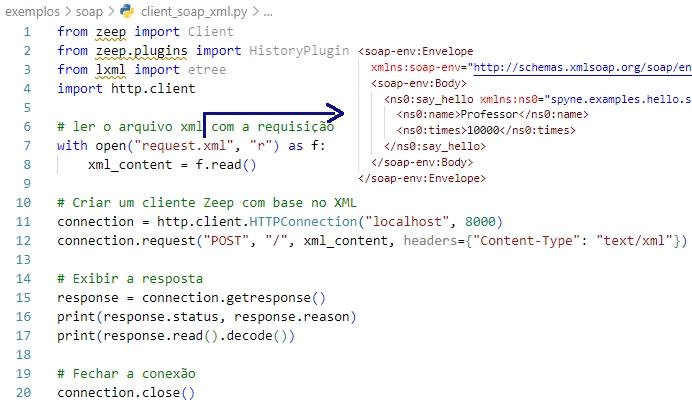
\includegraphics[width=0.9\linewidth]{client_xml.PNG}
		\caption{SOAP - Chamada Direta - Cliente}
		\label{fig:soap_client_xml}
	\end{figure}

\end{frame}

\begin{frame}[fragile]
	\frametitle{SOAP}
	\framesubtitle{Enviando XML para o Servidor via Postman}

	\begin{figure}
		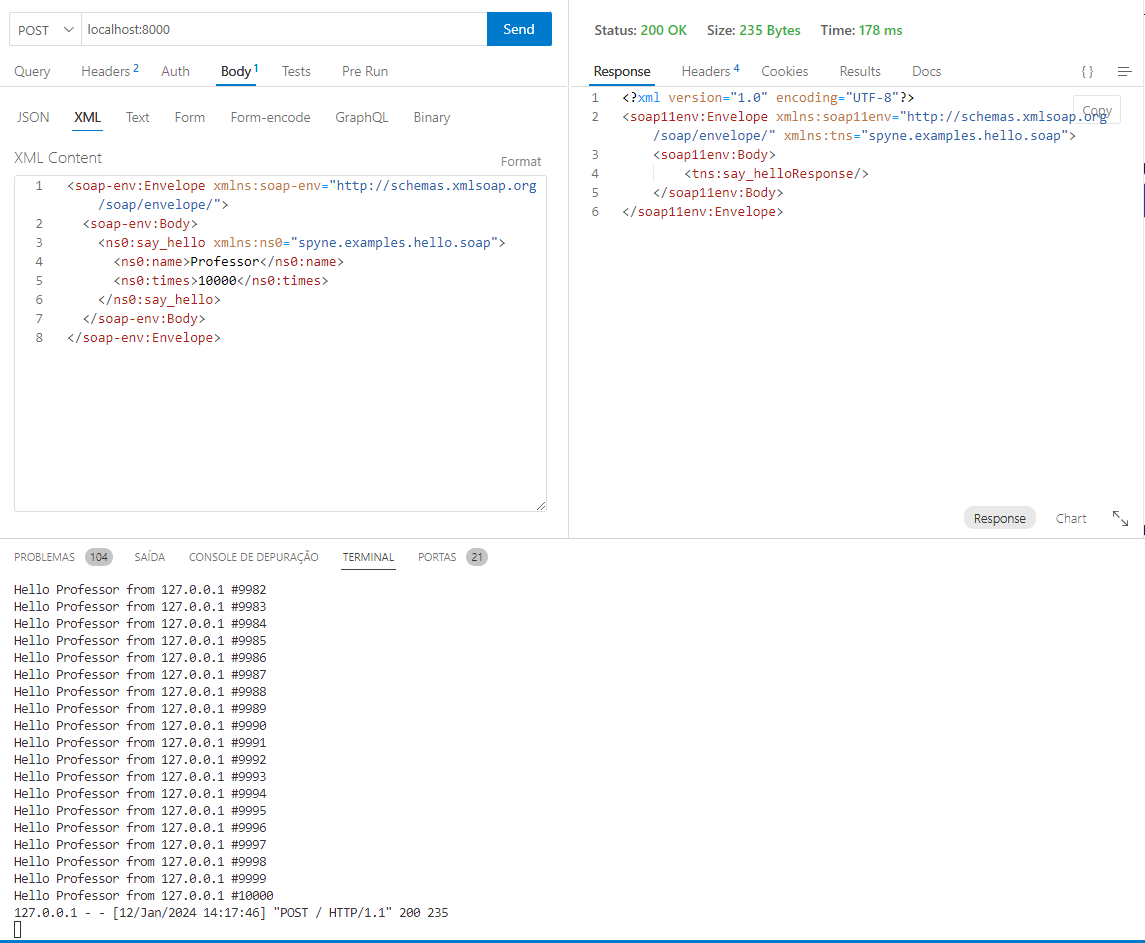
\includegraphics[width=0.7\linewidth]{soap_http_request_example.PNG}
		\caption{SOAP - Enviando XML}
		\label{fig:soap_server_xml_2}
	\end{figure}

\end{frame}

\subsection{Experimentos}

\begin{frame}
	\frametitle{Experimentos}
	\framesubtitle{Web Service}

	\begin{block}{Experimento 1}
		\begin{itemize}
			\item Crie um cliente SOAP para o Web Service
			      \href{http://www.dneonline.com/calculator.asmx?WSDL}{http://www.dneonline.com/calculator.asmx?WSDL}.
			      Escolha uma linguagem de programação de sua preferência.
		\end{itemize}
	\end{block}

	\begin{block}{Experimento 2}
		\begin{itemize}
			\item Crie um Web Service do tipo SOAP para calcular o MDC (Máximo Divisor Comum) de
			      uma imagem digital com largura e altura (x e y).
			\item Para implementar o servidor, use o WSDL
			      \href{https://gist.github.com/fabricioifc/bf6ccecd92d2aefc7362bdce5342f2c2}{disponível
				      aqui}.
			\item Implemente um cliente para testar o Web Service. Com a resposta do servidor,
			      calcule o Aspect Ratio da imagem usando a fórmula: $\text{Aspect Ratio} =
				      {x/MDC} : {y/MDC}$
			\item Peça para outro colega testar seu Web Service.
		\end{itemize}
	\end{block}

\end{frame}

\end{document}
